\begin{figure}
  \centering
  \begin{minipage}
    {0.45\linewidth}
    \centering
    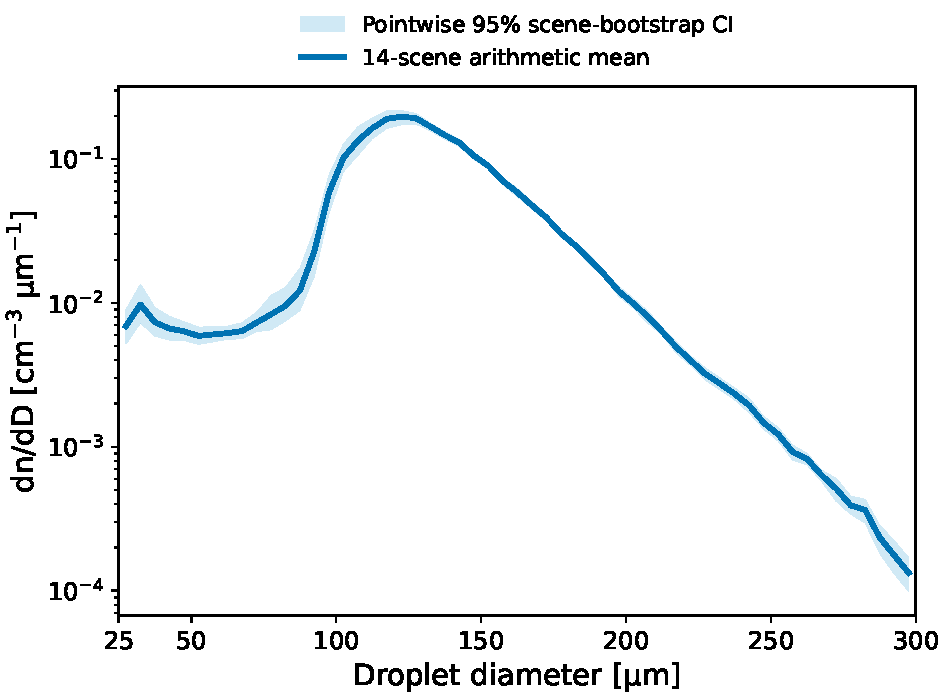
\includegraphics[width=0.98\linewidth]{figures/methods/particle_size_distribution_mean_ci_260715.pdf}
    \subcaption{
      Droplet number-density distribution
    }
  \end{minipage}
  \hspace{3mm}
  \begin{minipage}
    {0.48\linewidth}
    \centering
    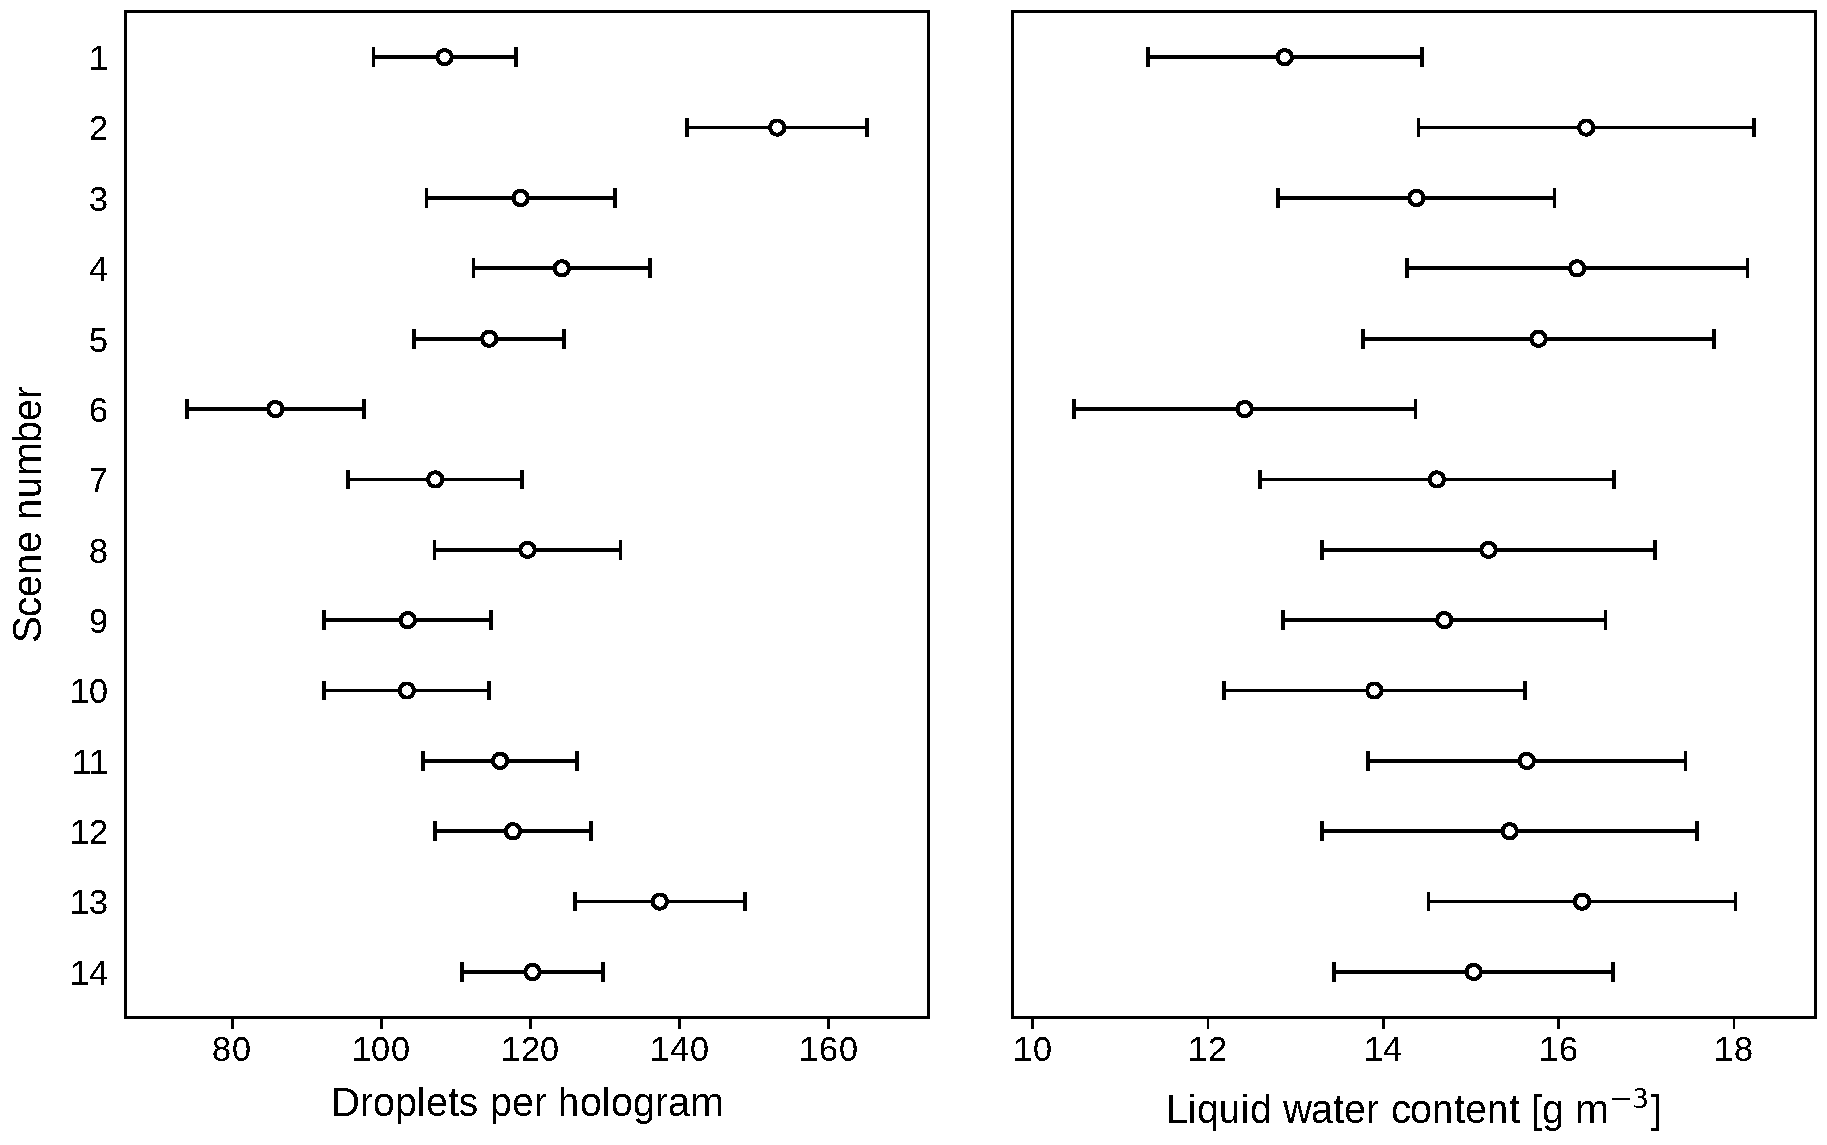
\includegraphics[width=0.98\linewidth]{figures/methods/particle_count_lwc_scene_summary.pdf}
    \subcaption{
      Droplet count per hologram and liquid water content
    }
  \end{minipage}
  \caption{
    Measured droplet population statistics for the 14 experimental sequences. (a) Droplet number-density distribution, \(dn/dD\), as a function of diameter \(D\). The solid curve is the arithmetic mean of the sequence-specific distributions, and the shaded region is the pointwise 95\% confidence interval obtained by resampling the sequences. (b) Droplet count per hologram and liquid water content for each sequence. Symbols indicate the sequence mean, and horizontal error bars indicate the sequence standard deviation.
  }
  \label{fig:exp_data_nd}
\end{figure}
